\chapter{Concept \& Design}

In this chapter we describe the research problem and our solution. Regarding the solution we discuss 
the ML aspects of this research and the architectural design to get the ML models running in a real-time
environment.

\section{Problem Statement}
The rise of online tracking techniques poses significant privacy concerns for users while browsing the web.
Traditional methods of tracking detection, such as static blacklists, are limited in their ability to adapt
to evolving tracking techniques in real-time. Although ML classifier have been developed to verify and support
the creation of TPLs there is no ML based blocking of malicious HTTP requests. Currently, all web extensions focused on blocking
ads and tracker use some kind of blocking list. As a result, there is a pressing need for an adaptive real-time application which
proves the concepts of ML based tracker detection and utilizes them in order to block tracking request while browsing the web.
\section{Solution}
In this thesis we present an AI driven web extension capable of blocking tracking requests in a real-time fashion and an approach on how
to continuously train this model and distribute it to our users. To create this kind of application many factors are important. In this 
section we elaborate on the AI model, the used frameworks and the overall application infrastructure.
\subsection{Model}
Developing a robust and effective real-time machine learning-based tracking detection application includes the crucial challenge
of selecting an appropriate ML model. The chosen model must have a high level of reliability and accuracy in identifying web
trackers. It is required to have the capability to identify tracking requests from the data available before the request is sent
to the server.

In addition to accurate tracking detection, the selected model needs to be able to predict very fast.
The application must be designed to operate within a web extension environment, where efficiency and responsiveness are important.
Quick prediction capabilities are essential to ensure that the model's execution does not introduce any detrimental impact on
the overall user experience.

Therefore, striking a balance between accuracy and efficiency is important when selecting the model for the real-time
tracking detection application. The model must possess the ability to analyze incoming data fast and make accurate predictions
in real-time, ensuring that tracking requests are identified and flagged promptly. By achieving this delicate balance, the application
can effectively protect user privacy without compromising the seamless browsing experience.

A promising ML model for this task has been proposed by Castell-Uroz et al. \cite{castell2020url}. For their classification the only thing
the model requires is the request URL. This model achieved an accuracy of 97\% which is solid for our use case.

Furthermore, Castell-Uroz et al. describe their approach of encoding the web request URL into numerical
representations ranging from 1 to 90. To streamline the input data, they restrict the input vector to 200 features.
In cases where a URL exceeds the 200-character limit, the initial characters are truncated. Conversely, if a URL
is shorter than the limit, the remaining positions in the input vector are padded with zeros from the left.
This encoding strategy ensures that the model effectively processes URL because Castell-Uroz et al. identified that the important
features for tracker detection likely to appear at the end of the URL string.
\begin{figure}[ht!]  
  \centering
  \begin{subfigure}[b]{.47\textwidth}
      \centering
      \includegraphics[width=\linewidth ]{images/model1.png}
      \caption{This figure shows the encoding of the feature vector for the first model. The feature vector includes 204 features. The first 200 features are reserved for the encoded URL
   string. The four following features include the frametype encoded from one to three, the HTTP method encoded from one to eight, the 
 request type encoded from one to twelve and the presence of the referrer header encoded from zero to one.}
      \label{fig:featModel1}
  \end{subfigure}
  \hfill
  \begin{subfigure}[b]{.47\textwidth}
      \centering
      \includegraphics[width=\linewidth, keepaspectratio]{images/model2.png}
      \caption{This figure shows the encoding of the feature vector for the second model. The feature vector includes 233 features. Similar to the 
        first model this model also uses the encoded request URL, frametype, HTTP method and request type. Additionally, this vector includes 30 characters
        of the request initiator URL.
      }
      \label{fig:featModel2}
  \end{subfigure}
  \label{}
  \caption{This figure shows the feature vector of the two ML models.}
\end{figure}  

However, it is important to note that there is additional information available prior to sending a request to the server.
To leverage this additional information, we have developed two distinct ML models while maintaining
the same underlying model structure, similar to the approach followed by Castell-Uroz et al.

For the first model, we have incorporated 204 features, as illustrated in Fig-\ref{fig:featModel1}. Consistent with Castell-Uroz et al.,
we have utilized the initial 200 features to encode the request URL. In addition to the URL, we have also encoded the frametype\footnote{frametype},
which can take one of three distinct values. Furthermore, we have encoded the HTTP method\footnote{method}, which can take
one of eight distinct values, the request type\footnote{type}, which can take one of twelve distinct values,
and lastly, the presence of the referrer header\footnote{referrer header}.

For the second model, we have incorporated 233 features, as illustrated in Fig-\ref{fig:featModel2}. Similar to the first model,
we use the encoded request URL, frametype, HTTP method and request type. However, we also encode
30 characters of the request initiator. The request initiator in this case is the first-party website which initiated the request. This 
initiator URL gets encoded like the request URL and added after the encoding of the request URL.

\begin{figure}[ht!]
  \begin{center}
    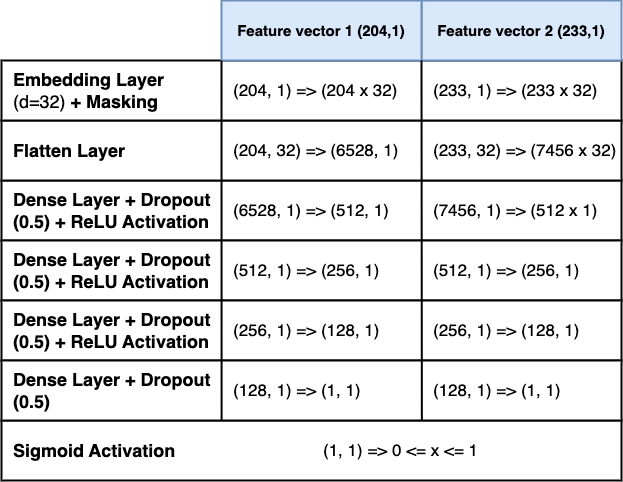
\includegraphics[width=0.7\textwidth]{images/DL.png}
  \end{center}
  \caption{This figure shows the deep learning model for both feature vectors. The different layers are shown on left column of the table. The input
  and output dimensions for each layer are shown in the other two columns.}
  \label{fig:modelStructure}
\end{figure}

By incorporating these additional features into our ML models, we aim to enhance the accuracy and effectiveness of
the tracking detection process, considering a broader range of contextual information associated with each request. 
Furthermore, every feature is known before a request is sent to the server and can be used to identify a tracking request
in real-time.

The deep neural network structure is almost identical to Castell-Uroz et al. \cite{castell2020url} and is illustrated in Fig-\ref{fig:modelStructure}.
The differences come from the different activation
function and the different input and output vector dimensions due to the different feature vectors. As Castell-Uroz et al. we use an embedding layer to reduce the bias between the numerical values of the embedded URL string. This embedded 
representation then gets flattened into a one dimensional vector and put into the four dense layers. Each dense layer has a dropout rate of 50\% to reduce
overfitting and a ReLU\footnote{Relu} activation function. The last dense layer gets activated by a Sigmoid\footnote{Sigmoid} function to generate an output
between zero and one.

By using the neural network structure of Castell-Uroz et al. we hope to achieve similar or better accuracy results with 
the newly crafted feature vector designs. However, it could be possible that the network architecture is not optimal
for the desired output and does not fit the different feature vectors. There is a chance that a better architecture could 
lead to a better accuracy result and therefore would better fit the real-time application of the model.



\subsection{Training-Data}
\subsection{Frameworks}
\subsection{Infrastructure}
\section{Methodology}
Literature Review
Empirical
- Classifier Performance
- Performance
- Quality of Experience
Design science






